\documentclass[aspectratio=169]{beamer}

% ------------------------------------------------
% Codificação e idioma
% ------------------------------------------------
\usepackage[utf8]{inputenc}
\usepackage[T1]{fontenc}
\usepackage[brazil]{babel}
\usepackage{amsmath, amssymb}
\usepackage{booktabs}
\usepackage{graphicx}

% ------------------------------------------------
% TikZ
% ------------------------------------------------
\usepackage{tikz}
\usetikzlibrary{positioning, arrows.meta, shapes.geometric}

% ------------------------------------------------
% Tema visual e esquema de cores
% ------------------------------------------------
\usetheme{Madrid}
\usecolortheme{seahorse}
\setbeamertemplate{navigation symbols}{}

% Ajuste sutil para espaçamento limpo em 16:9
\setbeamersize{text margin left=0.6cm, text margin right=0.6cm}

% ------------------------------------------------
% Informações da apresentação
% ------------------------------------------------
\title[Otimização de Cronogramas de Projeto]{
Otimização do Cronograma de Projetos de Arquitetura e Engenharia
}

\subtitle{
Modelagem RCPSP, Resolução Exata e Heurística, e Análise de Sensibilidade em um Empreendimento Real
}

\author[Grupo 2]{
\texorpdfstring{
Caio César Araújo Guimarães -- 2023422587 \\
Guilherme de Paula Oliveira -- 2025421294 \\
Thales Vasconcelos -- 2018019630 \\
Henrique Viana Lima de Oliveira -- 2023066543
}{
Caio César Araújo Guimarães; Guilherme de Paula Oliveira; Thales Vasconcelos; Henrique Viana Lima de Oliveira
}
}

\institute[UFMG]{
Universidade Federal de Minas Gerais (UFMG) \\
Pesquisa Operacional
}

\date{25 de novembro de 2026}

\begin{document}

% ================================================
% CAPA
% ================================================
\begin{frame}[plain]
    \titlepage
\end{frame}

% ================================================
% SLIDE 1 --- CONTEXTO E PERGUNTA DE PESQUISA
% ================================================
\section{Contextualização}

\begin{frame}{Contexto e pergunta de pesquisa}

\begin{columns}[T,onlytextwidth]

\begin{column}{0.51\textwidth}
\scriptsize
\begin{itemize}
    \setlength{\itemsep}{0.10cm}
    \item \textbf{Estudo de caso real:} coordenação do cronograma de \textbf{projeto} de um empreendimento residencial de grande porte.
    \item Envolve dezenas de equipes interdependentes: projetistas, análises do cliente, consultorias e aprovações.
    \item A \textbf{Arquitetura} conduz o ciclo: emite a base, as disciplinas desenvolvem sobre ela, o cliente analisa/compatibiliza e inicia-se uma nova revisão.
    \item \textbf{A dor prática:} cronogramas montados manualmente em fila criam \textbf{esperas ocultas}, alongando o prazo de liberação para a obra.
    \item Estrutura clássica de \textbf{RCPSP} (\emph{Resource-Constrained Project Scheduling Problem}).
\end{itemize}
\end{column}

\begin{column}{0.45\textwidth}
    \centering
    \footnotesize\textbf{Fluxo simplificado de dependências}

    \vspace{0.22cm}
    \resizebox{\linewidth}{!}{%
    \begin{tikzpicture}[
        node distance=0.22cm and 0.55cm,
        box/.style={rectangle, draw=blue!55!black, fill=blue!7, rounded corners=2pt,
                    font=\scriptsize, align=center, minimum width=1.65cm, minimum height=0.45cm},
        cli/.style={rectangle, draw=orange!75!black, fill=orange!15, rounded corners=2pt,
                    font=\scriptsize, align=center, minimum width=1.45cm, minimum height=0.58cm},
        fin/.style={rectangle, draw=green!50!black, fill=green!12, rounded corners=2pt,
                    font=\scriptsize, align=center, minimum width=1.55cm, minimum height=0.58cm},
        arr/.style={-{Stealth[length=4pt]}, thick, draw=black!65}
    ]
        \node[box] (arq) {Arquitetura\\(ARQ)};
        \node[box, right=0.55cm of arq, yshift=0.95cm] (est) {Estrutura / Fund.};
        \node[box, below=0.14cm of est] (inst) {Instalações / PCI};
        \node[box, below=0.14cm of inst] (cxo) {Caixilhos (CXO)};
        \node[box, below=0.14cm of cxo] (ari) {Interiores (ARI)};

        \node[cli, right=0.55cm of inst, yshift=-0.28cm] (anl) {Análise\\Cliente};
        \node[fin, right=0.45cm of anl] (comp) {Compatib.\\e Aprov.};

        \foreach \n in {est, inst, cxo, ari} {
            \draw[arr] (arq.east) -- (\n.west);
            \draw[arr] (\n.east) -- (anl.west);
        }
        \draw[arr] (anl.east) -- (comp.west);
    \end{tikzpicture}%
    }

    \vspace{0.22cm}
    \scriptsize\emph{Cada disciplina alterna emissões do projetista e análises do cliente até o fechamento da etapa.}
\end{column}

\end{columns}

\vfill

\begin{block}{Pergunta de pesquisa}
\scriptsize
Quanto é possível reduzir o prazo total do processo de projeto mantendo fixas as atividades, durações declaradas, equipes responsáveis e vínculos da base real?
\end{block}

\end{frame}

% ================================================
% SLIDE 2 --- INSTÂNCIA REAL (BASE R14) E MODELAGEM
% ================================================
\section{Instância real e modelagem}

\begin{frame}{Instância real anonimizada (base R14) e modelagem}

\begin{columns}[T,onlytextwidth]

\begin{column}{0.46\textwidth}
\begin{block}{O que é o R14 e o cenário atual}
\scriptsize
\begin{itemize}
    \setlength{\itemsep}{0.10cm}
    \item \textbf{Revisão R14:} revisão oficial do cronograma real do empreendimento, anonimizada para o estudo.
    \item \textbf{243 atividades reais.}
    \item \textbf{39 equipes/papéis} (projetistas, cliente e consultorias).
    \item \textbf{Prazo praticado: 310 dias úteis} (escala $0 \dots 309$).
\end{itemize}
\end{block}
\end{column}

\begin{column}{0.04\textwidth}\end{column}

\begin{column}{0.48\textwidth}
\begin{block}{Modelagem}
\scriptsize
\begin{itemize}
    \setlength{\itemsep}{0.07cm}
    \item \textbf{Duração ($d_a$):} intervalo início--entrega em dias úteis; \textbf{já inclui pausas internas} (não mede horas de esforço).
    \item \textbf{Capacidade ($R_k$):} máximo de atividades simultâneas, estimado pelo \textbf{pico observado} (ex.: ARQ = 6; Produto = 7).
    \item \textbf{TI com lag 0:} sucessora pode iniciar no dia da entrega; se compartilharem equipe, ambas contam no dia.
    \item \textbf{Calendário comum:} dias úteis consecutivos, sem feriados; replanejamento desde o dia 0.
\end{itemize}
\end{block}
\end{column}

\end{columns}

\vspace{0.22cm}

\begin{alertblock}{Descoberta no R14: duas versões da base}
\scriptsize
\textbf{27 atividades sem predecessora} começaram tarde (dias 41--220) por dependerem de etapas anteriores do \textbf{Estudo Preliminar de Arquitetura}. Por isso analisamos: \textbf{(1) com liberações} (presas às datas praticadas $\rightarrow$ cenário realista) e \textbf{(2) largadas livres} (dia 0 $\rightarrow$ limite teórico).
\end{alertblock}

\end{frame}

% ================================================
% SLIDE 3 --- MODELO MATEMÁTICO COMPLETO
% ================================================
\section{Modelo matemático}

\begin{frame}{Modelo de Programação Linear Inteira Mista (indexado no tempo)}

\begin{columns}[T,onlytextwidth]

\begin{column}{0.46\textwidth}
\begin{block}{Descrição das variáveis e símbolos}
\fontsize{6.3pt}{7.6pt}\selectfont
\centering
\renewcommand{\arraystretch}{1.12}
\begin{tabular}{@{}ll@{}}
\toprule
\textbf{Símbolo} & \textbf{Significado} \\
\midrule
$x_{a\tau} \in \{0,1\}$ & 1 se atividade $a$ inicia no dia $\tau$; 0 c.c. \\
$C_{\max} \ge 0$ & Prazo total do projeto (\emph{makespan}) \\
$S_a$ & Dia de início de $a$ ($\sum_{\tau \in T_a} \tau x_{a\tau}$) \\
$F_a$ & Dia de entrega de $a$ ($S_a + \max(d_a,1) - 1$) \\
$d_a$ & Duração da atividade $a$ (dias úteis) \\
$q_{ak} \in \{0,1\}$ & 1 se equipe $k$ participa de $a$; 0 c.c. \\
$R_k$ & Capacidade da equipe $k$ (ativ. simult.) \\
$\ell_e$ & Espera (\emph{lag}) do vínculo $e=(i,j)$ \\
$r_a$ & Data de liberação de $a$ (cenário realista) \\
$A, A^+, A^L$ & Atividades: todas, $d_a > 0$, c/ liberação \\
$K, T, T_a$ & Equipes, dias ($0 \ldots H{-}1$) e inícios válidos \\
TI/II/TT/IT & Vínculos Término/Início entre $i$ e $j$ \\
\bottomrule
\end{tabular}
\end{block}
\end{column}

\begin{column}{0.04\textwidth}\end{column}

\begin{column}{0.48\textwidth}
\begin{block}{Função objetivo e restrições}
\fontsize{6.6pt}{7.8pt}\selectfont
\setlength{\jot}{1.5pt}
\vspace{-0.26cm}
\begin{align*}
\min\quad & C_{\max} \\
\text{s.a.}\quad
& \sum_{\tau \in T_a} x_{a\tau} = 1, && \forall a \in A \;\; \text{(início único)} \\
& S_j \ge F_i + \ell_e \;\; (\text{TI}), && S_j \ge S_i + \ell_e \;\; (\text{II}) \\
& F_j \ge F_i + \ell_e \;\; (\text{TT}), && F_j \ge S_i + \ell_e \;\; (\text{IT}) \\
& \sum_{a \in A^+} q_{ak} \!\!\!\sum_{\substack{\tau \in T_a \\ t-d_a+1 \le \tau \le t}}\!\!\! x_{a\tau} \le R_k, && \forall k \in K,\; t \in T \\
& C_{\max} \ge F_a + 1, && \forall a \in A \;\; \text{(makespan)} \\
& S_a \ge r_a, && \forall a \in A^L \;\; \text{(liberações)}
\end{align*}
\end{block}

\vspace{0.08cm}

\begin{block}{Porte na base completa ($H = 310$)}
\fontsize{6.5pt}{7.8pt}\selectfont
\textbf{72.381} binárias + $C_{\max}$ \;\;$\bullet$\;\; \textbf{13.584} restrições \;\;$\bullet$\;\; \textbf{1,69 M} não nulos.
\end{block}
\end{column}

\end{columns}

\end{frame}

% ================================================
% SLIDE 4 --- PIPELINE REVISADA E MÉTODOS
% ================================================
\section{Abordagem e pipeline}

\begin{frame}{Pipeline de solução e complementaridade dos métodos}

\centering
\resizebox{\textwidth}{!}{%
\begin{tikzpicture}[
    node distance=0.35cm,
    stepbox/.style={rectangle, draw=blue!55!black, fill=blue!7, rounded corners=3pt,
                    font=\scriptsize, align=center, text width=2.25cm, minimum height=0.95cm},
    methbox/.style={rectangle, draw=orange!75!black, fill=orange!12, rounded corners=3pt,
                    font=\scriptsize, align=center, text width=2.55cm, minimum height=0.95cm},
    valbox/.style={rectangle, draw=green!50!black, fill=green!10, rounded corners=3pt,
                   font=\scriptsize, align=center, text width=2.25cm, minimum height=0.95cm},
    arr/.style={-{Stealth[length=5pt]}, thick, draw=black!70}
]
    \node[stepbox] (s1) {\textbf{1. Auditoria}\\Integridade, ciclos e referência viável};
    \node[stepbox, right=0.38cm of s1] (s2) {\textbf{2. Limite Inferior}\\CPM sem equipes gera $LB$ exato};
    \node[methbox, right=0.38cm of s2] (s3) {\textbf{3. Dois Métodos}\\(a) PLIM no CBC\\(b) Serial SGS};
    \node[valbox, right=0.38cm of s3] (s4) {\textbf{4. Validação}\\Confere vínculos, equipes e $UB = LB$};
    \node[stepbox, right=0.38cm of s4] (s5) {\textbf{5. Sensibilidade}\\Reotimiza equipes, durações e zonas};

    \draw[arr] (s1) -- (s2);
    \draw[arr] (s2) -- (s3);
    \draw[arr] (s3) -- (s4);
    \draw[arr] (s4) -- (s5);
\end{tikzpicture}%
}

\vspace{0.10cm}

\begin{columns}[T,onlytextwidth]

\begin{column}{0.46\textwidth}
\begin{block}{Método (a): Exato --- PLIM (PuLP + CBC)}
\fontsize{6.8pt}{8.2pt}\selectfont
\begin{itemize}
    \setlength{\itemsep}{0.07cm}
    \item Resolve a formulação indexada no tempo via \textbf{Branch-and-Cut}.
    \item Recebe o cronograma praticado (310 d) como \textbf{\emph{warm start}} (ponto de partida viável).
    \item \textbf{Força:} prova o ótimo mesmo quando a \textbf{capacidade das equipes trava o prazo} (instância pequena).
    \item \textbf{Limite:} com 72.381 binárias, o nó raiz consome o tempo e o solver não fecha o gap na base completa.
\end{itemize}
\end{block}
\end{column}

\begin{column}{0.04\textwidth}\end{column}

\begin{column}{0.48\textwidth}
\begin{block}{Método (b): Construtivo --- CPM + Serial SGS}
\fontsize{6.8pt}{8.2pt}\selectfont
\begin{itemize}
    \setlength{\itemsep}{0.05cm}
    \item \textbf{Montagem (Serial SGS):} ordena atividades por prioridade e aloca uma a uma no \textbf{primeiro dia livre} (vínculos + equipes), gerando um prazo viável (\textbf{$UB$}, limite superior).
    \item \textbf{Mínimo teórico (CPM):} calcula a maior cadeia de dependências sem limite de equipe, gerando o \textbf{limite inferior ($LB$)}.
    \item \textbf{Prova de ótimo ($UB = LB$):} se o prazo viável ($UB$) empata com o mínimo teórico ($LB$), não existe solução menor (\textbf{gap = 0\%}).
    \item \textbf{Validação independente:} checa automaticamente vínculos e equipes.
\end{itemize}
\end{block}
\end{column}

\end{columns}

\end{frame}

% ================================================
% SLIDE 5 --- RESULTADOS PRINCIPAIS (PRAZOS E MÉTODOS)
% ================================================
\section{Resultados}

\begin{frame}{Resultados principais: redução de prazo e métodos}

\begin{columns}[T,onlytextwidth]

\begin{column}{0.54\textwidth}
    \centering
    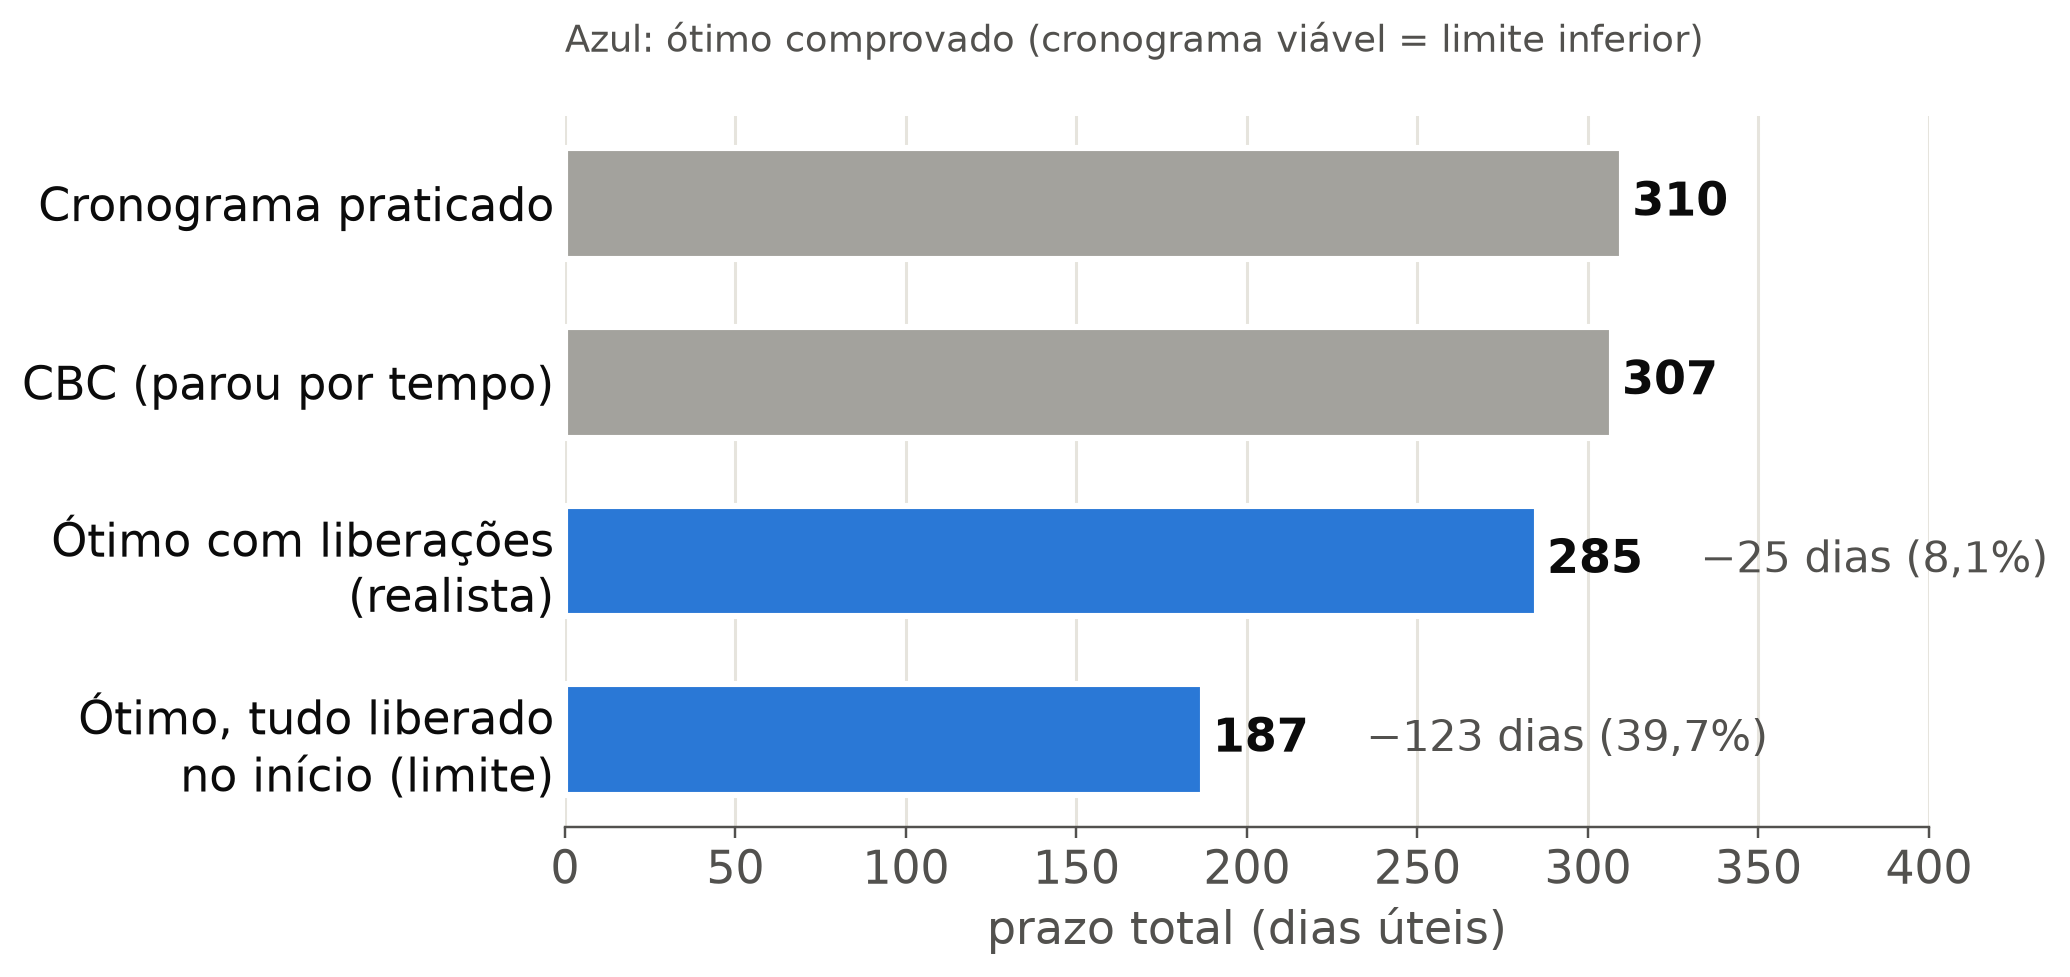
\includegraphics[width=\textwidth]{figuras/01-prazos.png}
\end{column}

\begin{column}{0.42\textwidth}
\scriptsize
\begin{block}{Comparação entre métodos}
\centering
\resizebox{\textwidth}{!}{
\begin{tabular}{llrrrl}
\toprule
Instância & Método & UB & LB & Tempo & Situação \\
\midrule
Pequena  & CBC        & 45  & 45  & 1,4 s   & ótimo \\
(12 atv.) & CPM + SGS  & 45  & 44  & $<$0,1 s & viável \\
\midrule
Completa & Praticado  & 310 & --  & --      & ref. \\
(243 atv.) & CBC (WS)   & 307 & 187 & 36 min  & gap 39\% \\
         & SGS (lib.) & \textbf{285} & \textbf{285} & 0,04 s  & \textbf{ótimo} \\
         & SGS (livre)& \textbf{187} & \textbf{187} & 0,25 s  & \textbf{ótimo} \\
\bottomrule
\end{tabular}
}
\end{block}

\vspace{0.08cm}

\begin{itemize}
    \setlength{\itemsep}{0.08cm}
    \item \textbf{Ganho realista:} \textbf{310 $\rightarrow$ 285 dias} (\textbf{$-$25 dias / $-$8,1\%}), ótimo comprovado apenas reordenando inícios.
    \item \textbf{Diferença 285 vs. 187 (98 dias):} mede o peso da espera pelo Estudo Preliminar de ARQ.
    \item \textbf{Complementaridade:} CBC prova na pequena (capacidade ativa); CPM + SGS prova na completa em $<$1 s.
\end{itemize}
\end{column}

\end{columns}

\end{frame}

% ================================================
% SLIDE 6 --- O QUE LIMITA O PRAZO (EQUIPES x CADEIA CRÍTICA)
% ================================================
\begin{frame}{O que limita o prazo: cadeia crítica, não tamanho das equipes}

\begin{columns}[T,onlytextwidth]

\begin{column}{0.43\textwidth}
    \centering
    \footnotesize\textbf{Efeito de variar a capacidade das equipes}
    \vspace{0.08cm}

    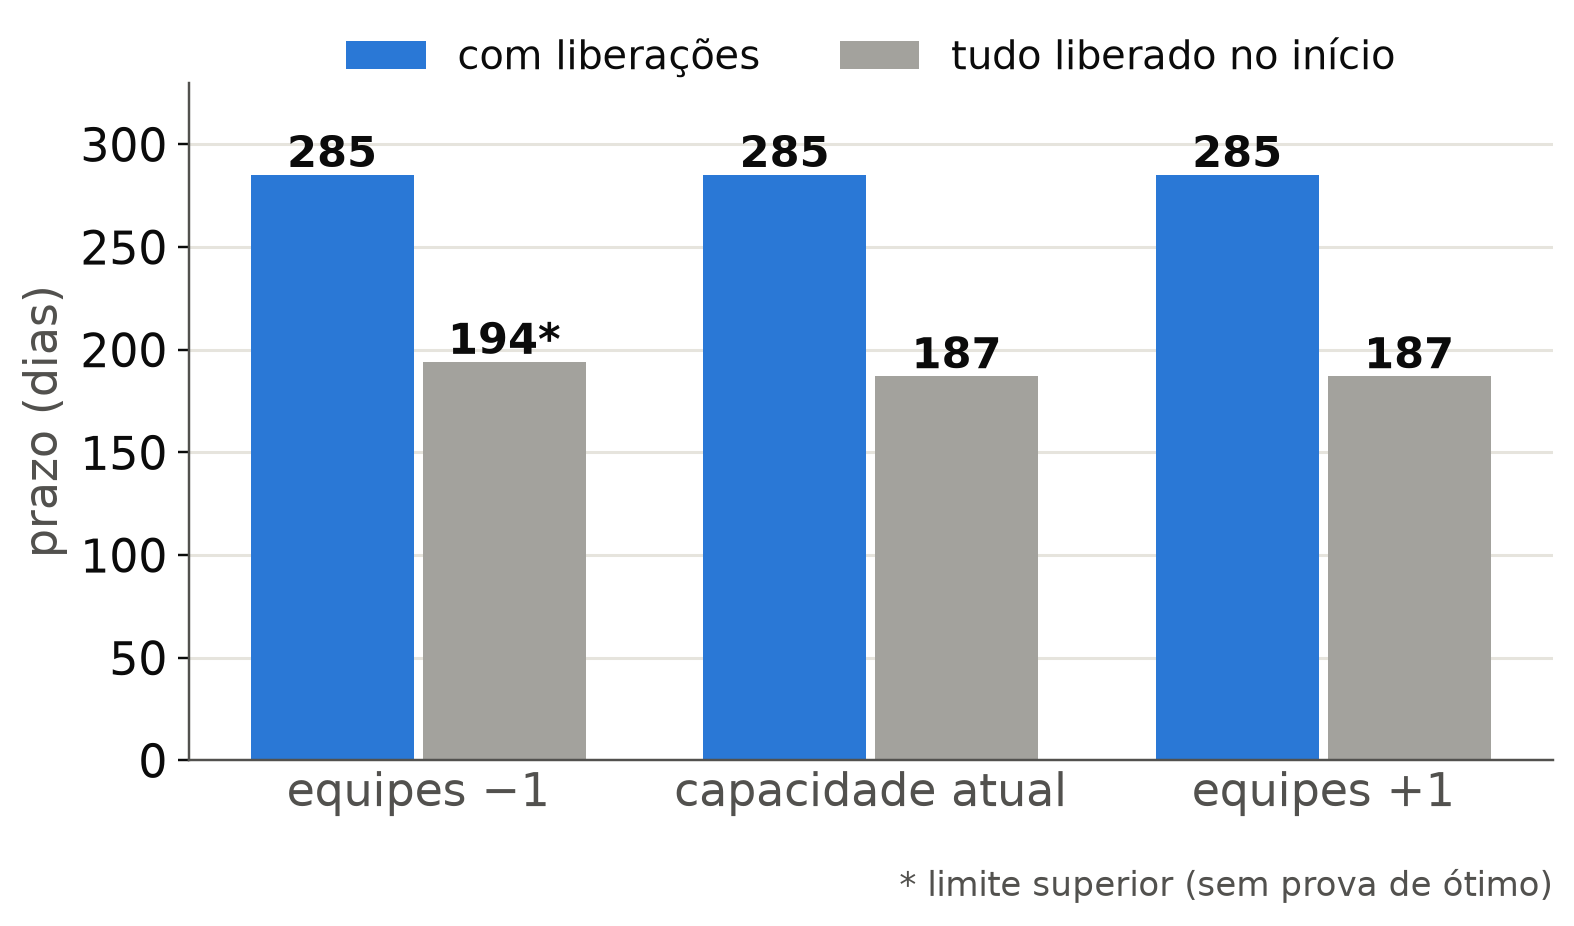
\includegraphics[width=0.92\textwidth]{figuras/05-equipes.png}

    \vspace{0.08cm}
    \scriptsize
    \begin{block}{Achado contraintuitivo}
    A restrição de capacidade \textbf{não está ativa no ótimo} (preço-sombra zero). Aumentar ou reduzir 1 frente em todas as equipes mantém o prazo em \textbf{285 dias}. \textbf{Contratar mais gente não reduz o prazo.}
    \end{block}
\end{column}

\begin{column}{0.53\textwidth}
    \centering
    \footnotesize\textbf{Cadeia crítica realista (14 atividades, 285 dias)}
    \vspace{0.08cm}

    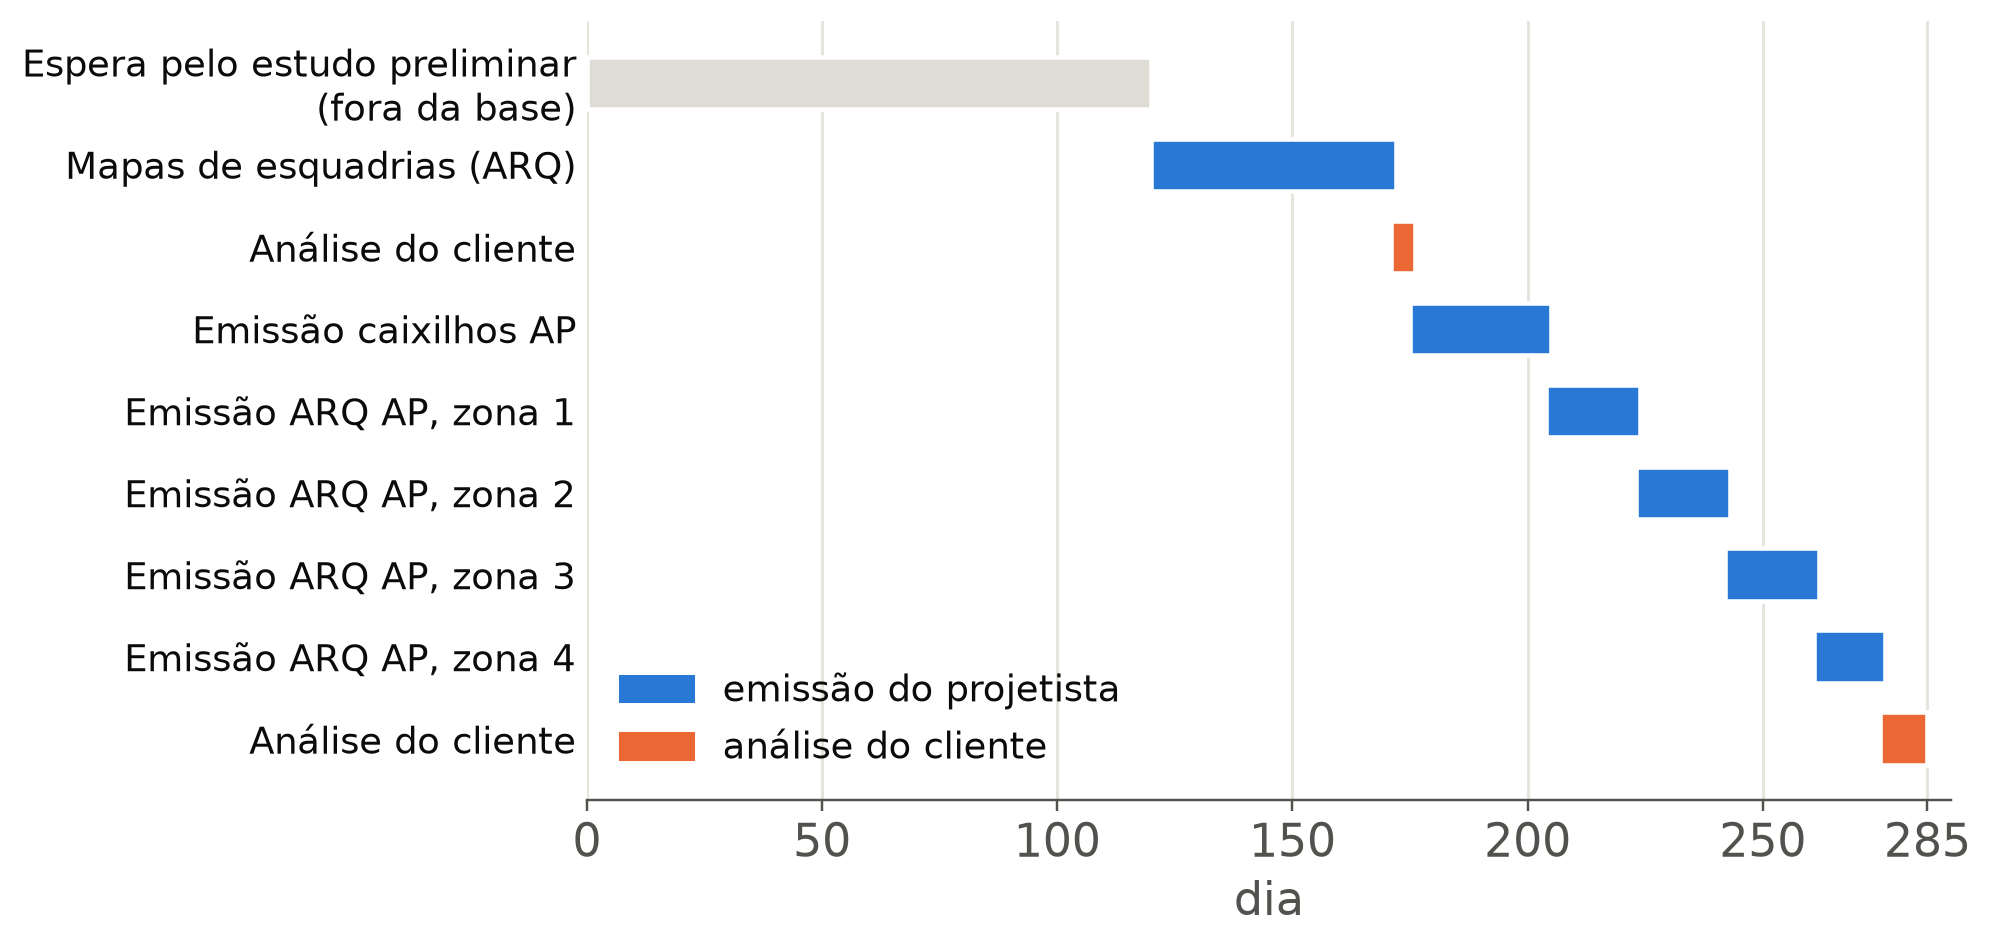
\includegraphics[width=0.88\textwidth]{figuras/04-cadeia-285.png}

    \vspace{0.06cm}
    \fontsize{6.8pt}{8.2pt}\selectfont
    \begin{itemize}
        \setlength{\itemsep}{0.04cm}
        \item \textbf{Cadeia crítica:} sequência de atividades encadeadas \textbf{sem folga} que dita o prazo final --- atrasar 1 dia nela atrasa toda a entrega.
        \item \textbf{Ciclo de Anteprojeto (AP) --- Arquitetura e Caixilhos:} a Arquitetura emite os \textbf{mapas de esquadrias} (portas e janelas, 52 d); \textbf{Caixilhos} projeta as esquadrias sobre esse mapa (30 d); depois a Arquitetura fecha o AP final das 4 zonas em sequência (75 d).
        \item Sem paralelismo (1 frente/equipe), o prazo iria a $\approx$614 dias; as frentes atuais já bastam.
    \end{itemize}
\end{column}

\end{columns}

\end{frame}

% ================================================
% SLIDE 7 --- ANÁLISE DE SENSIBILIDADE E PROPOSTAS
% ================================================
\begin{frame}{Análise de sensibilidade: onde agir para ganhar mais prazo}

\begin{columns}[T,onlytextwidth]

\begin{column}{0.49\textwidth}
    \centering
    \footnotesize\textbf{Redução sobre a base realista (285 dias)}
    \vspace{0.1cm}
    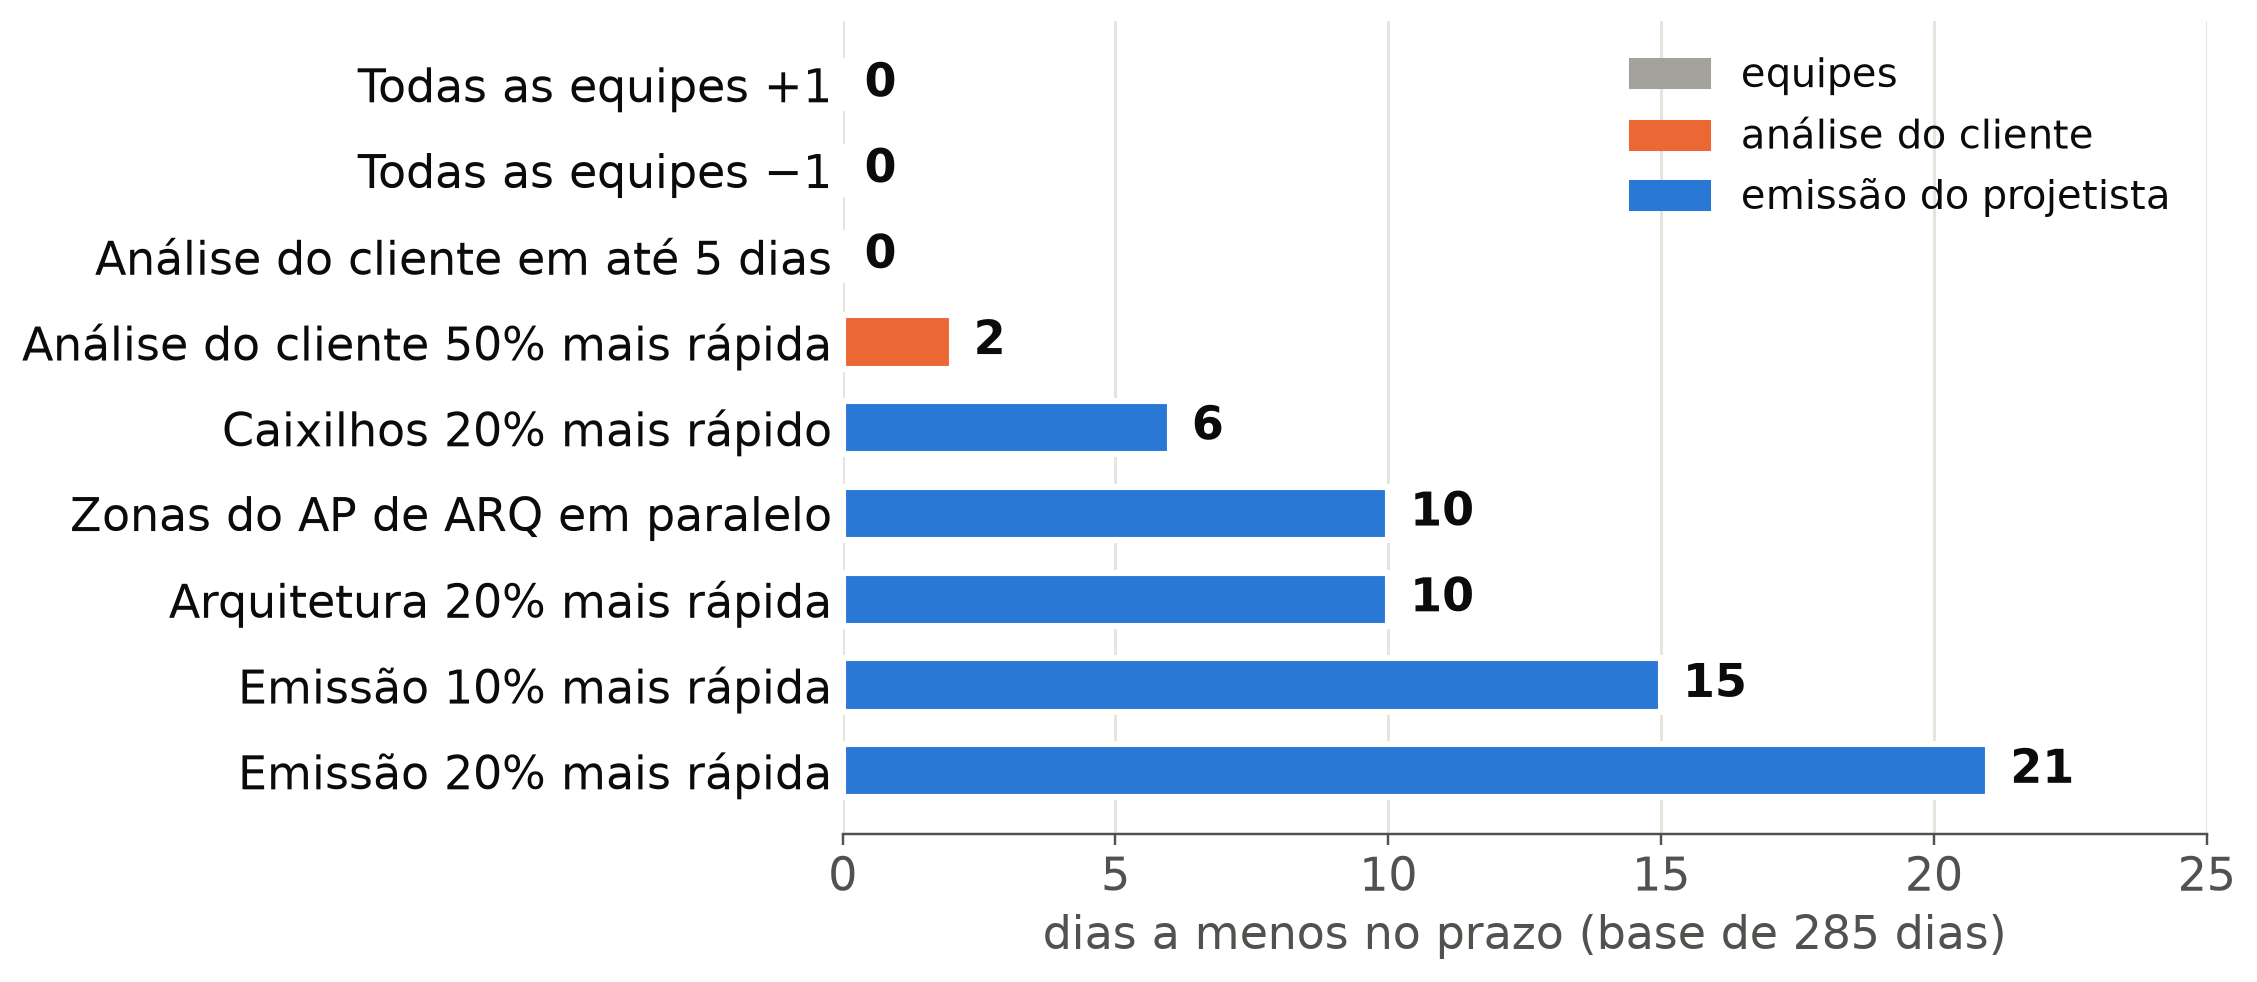
\includegraphics[width=\textwidth]{figuras/02-sensibilidade-285.png}
\end{column}

\begin{column}{0.46\textwidth}
    \centering
    \footnotesize\textbf{Emissão do projetista $\times$ Análise do cliente}
    \vspace{0.1cm}
    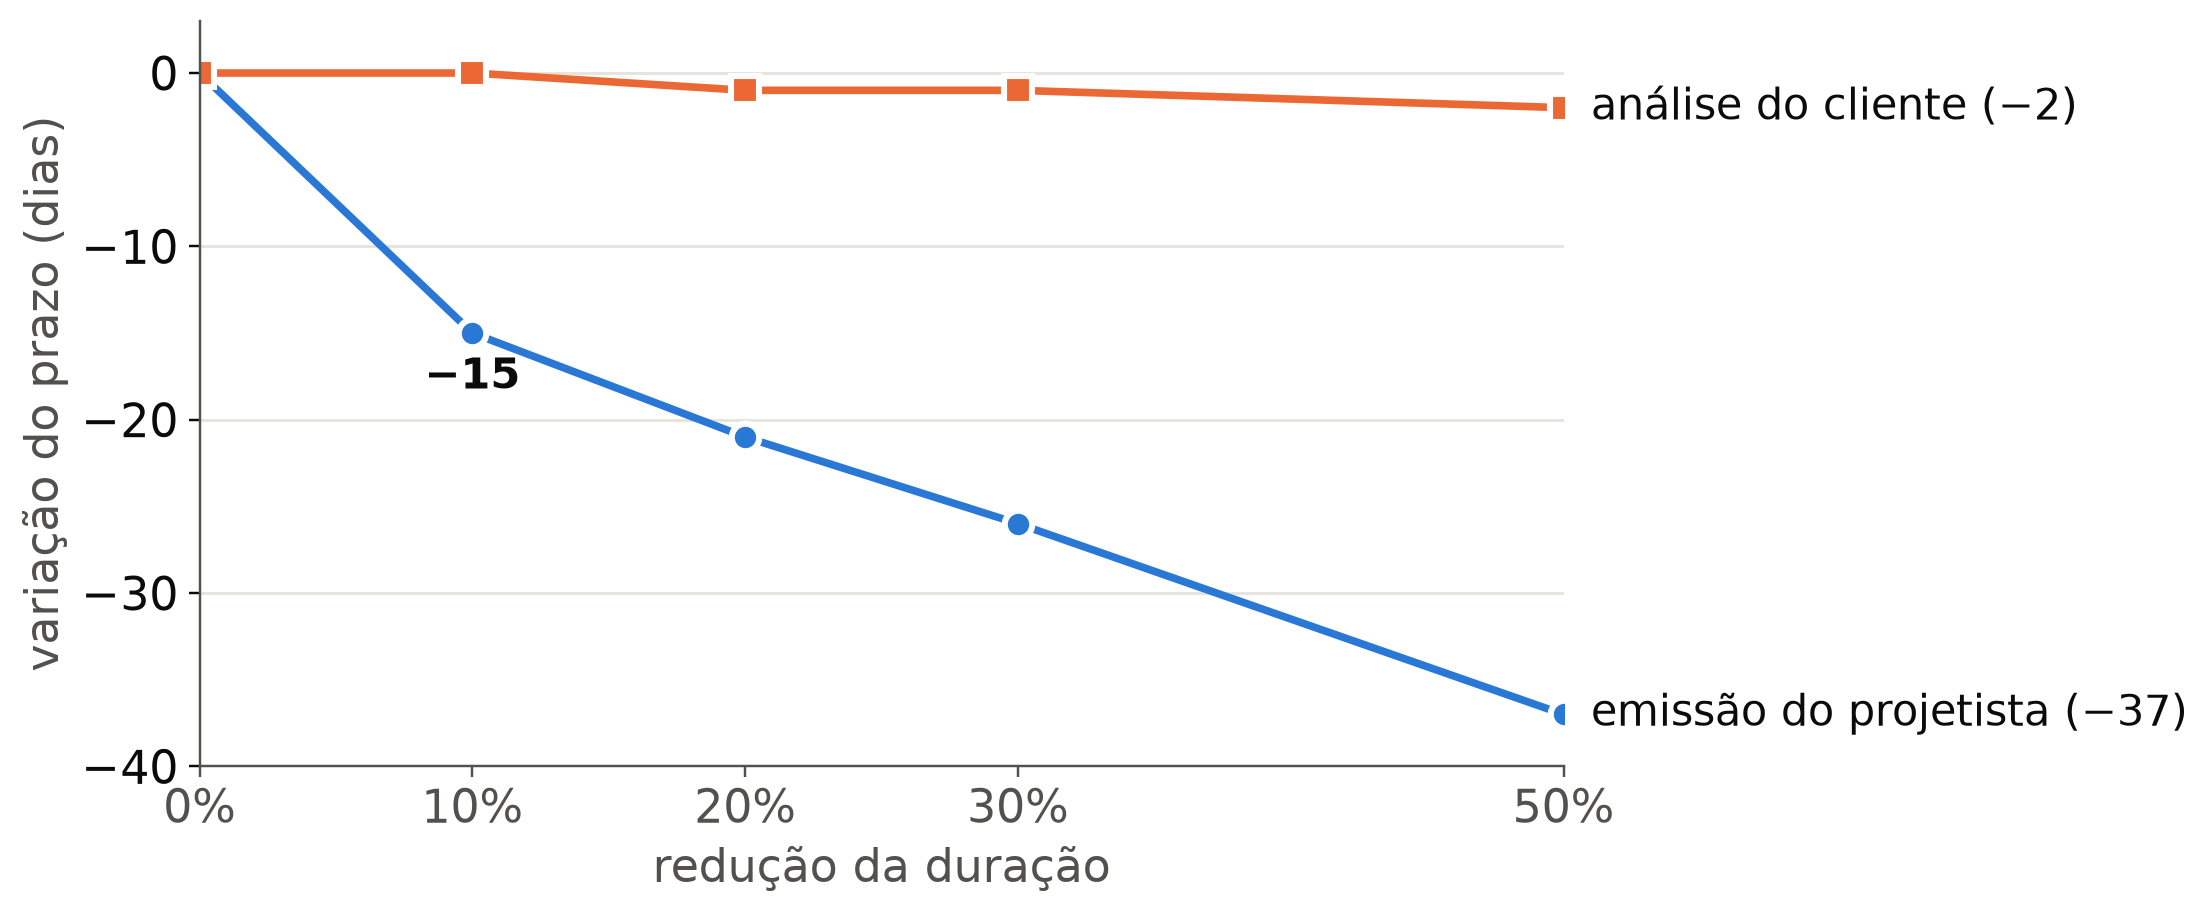
\includegraphics[width=\textwidth]{figuras/03-emissao-x-analise.png}
\end{column}

\end{columns}

\vspace{0.16cm}

\begin{block}{Alavancas gerenciais indicadas pelos dados}
\scriptsize
\begin{itemize}
    \setlength{\itemsep}{0.06cm}
    \item \textbf{A alavanca é a emissão do projetista, não a análise do cliente:} emitir \textbf{10\%} mais rápido ganha \textbf{$-$15 dias}; cortar a análise do cliente pela metade (\textbf{50\%}) ganha apenas \textbf{$-$2 dias} (SLA de 5 dias ganha 0).
    \item \textbf{Agir só na cadeia crítica:} acelerar ARQ em 20\% vale \textbf{$-$10 dias} e Caixilhos vale \textbf{$-$6 dias}; acelerar Interiores em 20\% vale \textbf{0 dia}. Padronização e automação BIM (ex.: mapa de esquadrias) devem mirar a cadeia crítica.
    \item \textbf{Paralelizar zonas do AP final de ARQ:} tratar as 4 zonas em paralelo (quando não há dependência técnica) reduz \textbf{$-$10 dias}.
\end{itemize}
\end{block}

\end{frame}

% ================================================
% SLIDE 8 --- LIMITAÇÕES E TRABALHOS FUTUROS
% ================================================
\section{Limitações e conclusões}

\begin{frame}{Limitações do estudo e trabalhos futuros}

\begin{columns}[T,onlytextwidth]

\begin{column}{0.47\textwidth}
\begin{block}{Limitações (transparência metodológica)}
\scriptsize
\begin{itemize}
    \setlength{\itemsep}{0.09cm}
    \item \textbf{Cobertura da base R14:} verificar melhor a cobertura da base quanto às etapas iniciais do Estudo Preliminar (representadas de forma conservadora pelas datas de liberação) e aos 59 vínculos ajustados na preparação.
    \item \textbf{Vínculo ausente na compatibilização:} restaurado em teste, muda o limite livre de 187 para 196 dias e \textbf{não altera o ótimo realista de 285 dias}.
    \item \textbf{Capacidades estimadas} pelo pico observado no praticado (porém a conclusão é robusta: $\pm 1$ frente não muda os 285 dias).
    \item \textbf{Durações fixas e calendário abstrato:} sem incerteza, sem feriados por equipe; replanejamento parte do dia 0.
\end{itemize}
\end{block}
\end{column}

\begin{column}{0.04\textwidth}\end{column}

\begin{column}{0.47\textwidth}
\begin{block}{Trabalhos futuros e implicações práticas}
\scriptsize
\begin{itemize}
    \setlength{\itemsep}{0.09cm}
    \item \textbf{Incluir o Estudo Preliminar na base:} permite medir o ganho de liberar a base de ARQ em pacotes por torre (atacando a diferença entre 285 e 187 dias).
    \item \textbf{Modelar revisões como decisão:} tratar a redução de ciclos de revisão via briefing mais fechado e alinhamento prévio.
    \item \textbf{Calendários e incerteza:} incorporar calendários específicos por equipe e otimização robusta para variabilidade de durações.
    \item \textbf{Hibridização (SGS $\rightarrow$ CBC):} usar o cronograma heurístico como \emph{warm start} do solver em instâncias onde a capacidade esteja ativa.
\end{itemize}
\end{block}
\end{column}

\end{columns}

\end{frame}

% ================================================
% SLIDE 9 --- CONCLUSÕES
% ================================================
\begin{frame}{Conclusões}

\begin{block}{Principais respostas do estudo}
\footnotesize
\begin{itemize}
    \setlength{\itemsep}{0.18cm}
    \item \textbf{Ganho real apenas por reordenação:} mantendo as mesmas atividades, durações, vínculos e equipes, o prazo cai de \textbf{310 para 285 dias úteis ($-$25 dias / $-$8,1\%)} com ótimo global comprovado respeitando as liberações reais --- e até \textbf{187 dias ($-$39,7\%)} no limite sem espera pelo Estudo Preliminar.
    \item \textbf{Diagnóstico gerencial claro:} o gargalo do empreendimento está na \textbf{cadeia crítica de precedências e emissões} (Arquitetura e Caixilhos), e \textbf{não na capacidade das equipes}. Contratar mais frentes não reduz o prazo; padronização BIM focada na cadeia crítica e paralelismo de zonas geram de 10 a 21 dias adicionais.
    \item \textbf{Complementaridade de métodos em PO:} a PLIM indexada no tempo (CBC) prova o ótimo quando a capacidade restringe o prazo (instância pequena), enquanto a combinação \textbf{CPM + Serial SGS} resolve a base completa em menos de 1 segundo com prova de otimalidade ($UB = LB$) e validação independente.
\end{itemize}
\end{block}

\vfill

\begin{center}
    \small\textbf{Mensagem final:} otimizar cronogramas de projeto não exige mais pessoas --- exige enxergar onde estão as folgas e atacar a cadeia que realmente comanda o prazo.
\end{center}

\end{frame}

% ================================================
% SLIDE 10 --- REFERÊNCIAS BIBLIOGRÁFICAS
% ================================================
\section{Referências}

\begin{frame}{Referências bibliográficas}

\scriptsize
\begin{itemize}
    \setlength{\itemsep}{0.15cm}
    \item \textbf{Ding, H., Zhuang, C., \& Liu, J. (2023).} \emph{Extensions of the resource-constrained project scheduling problem.} Automation in Construction, 153, 104958.
    \\ \textcolor{black!70}{Base conceitual do RCPSP, classificação das extensões e justificativa conjunta de precedências e recursos.}

    \item \textbf{Kong, F., \& Dou, D. (2020).} \emph{RCPSP with Combined Precedence Relations and Resource Calendars.} Journal of Construction Engineering and Management, 146(12).
    \\ \textcolor{black!70}{Fundamentação dos quatro tipos de precedência (TI, II, TT, IT) em projetos de construção civil.}

    \item \textbf{Colares, F. S. (2010).} \emph{Alocação de Equipes e Desenvolvimento de Cronogramas em Projetos de Software Utilizando Otimização.} Dissertação de Mestrado, UFMG.
    \\ \textcolor{black!70}{Ponte entre sequenciamento em projetos de software e engenharia, e análise de recursos versus prazo.}

    \item \textbf{Pass-Lanneau, A., Bendotti, P., \& Brunod-Indrigo, P. (2024).} \emph{Exact and heuristic methods for Anchor-Robust and Adjustable-Robust RCPSP.} Annals of Operations Research, 337, 649--682.
    \\ \textcolor{black!70}{Referência para rigor na avaliação computacional ($LB$, $UB$, gap) e discussão de durações fixas vs. incerteza.}

    \item \textbf{Procopio, R. et al. (2025).} \emph{Alocação ótima de tarefas em equipes Scrum usando Programação Linear Inteira.} ENMC/ECTM.
    \\ \textcolor{black!70}{Referência de estruturação e exposição de modelos de Programação Linear Inteira aplicados a equipes.}
\end{itemize}

\vfill
\begin{center}
    \normalsize\textbf{Obrigado! Dúvidas?}
\end{center}

\end{frame}

\end{document}
